\chapter{连接量子多体伤痕与非热化严格可解极限}\label{chap:ETH}

孤立系统的热化在理解宏观系统的量子统计描述中扮演重要的角色。对于仅有局域相互作用的哈密顿量,本征热化假说被提出用来给出孤立系统热化的解释。目前为止对此假说的论证主要集中于数值模拟。但是人们目前还不严格清楚其适用的范围。有趣的的是在一些特殊体系中,本征热化假说完全失效,称为强违背本征热化假说体系,其中以量子可积系统与多体局域化系统最为典型。随着研究者对此假说认识的不断加强,依赖于初态选取的弱违背本征热化假说体系被发现:考虑同一孤立体系,从某些初态出发会热化,但是从另外一些初态出发则不会热化。在本章中,我们选择固定的初态如$|Z_2\rangle$出发,探索整个参数区间下带有纵场的横场伊辛模型的热化相图,并讨论发现的不同热化区域及其背后的物理解释。我们在~\ref{4sec:intro}~节中给出此研究的动机,~\ref{4sec:method}~节中讨论涉及的模型和方法,~\ref{4sec:result}~节中针对得到的热化相图做分析,我们主要发现了多体伤痕附近的非热化行为,并与严格可解极限做了联系,最后我们还发现了基态附近的弱热化行为。在~\ref{4sec:sum}~节我们总结目前的结果并做简要的小结。

\section{引言}\label{4sec:intro}
在热力学平衡态的角度,量子统计力学给出了宏观物体的热力学描述。仅用几个参数就可以描述处于热力学平衡态的宏观数目自由度的体系。而量子统计力学中一个关键原理即是等概率原理——具有相同能量的微观量子态在热力学平衡态分布中出现的几率相同。基于此原理,我们引入微正则系综来描述平衡态分布,为了与实验体系比较,我们又引入了在热力学极限下与之等价的正则系综与巨正则系综。但是在另一个角度,根据量子力学基本定律,我们知道孤立量子体系的演化为幺正的。如果我们准备一个孤立系统处于初态$|\psi(t=0)\rangle$,初态在不同本征态上的投影几率为$\langle E_\alpha|\psi(t=0)\rangle$,这一几率在幺正演化下是不变的。对于一个系统的长时间平均测量,其观测值似乎在初态决定的时候就已经决定了,看似是初态依赖的,这与统计力学中假设的时间平均等价于等概率系综平均乍一看是矛盾的。为了解决这一矛盾,Deutsch J M\cite{Deutsch1991quantum}与Srednicki M\cite{Srednicki1994chaos}分别独立地提出了本征热化假说,其核心思想为当我们观测一个孤立系统的局域可观测量时,系统的剩余部分作为这个局域自由度的热库,这一热接触的温度由系统总的能量给出。这一假说在后续很多体系的数值试验中得到验证。具有很强的普适性。更加形式化的讨论以及数值证据可以参见我们~\ref{1sec:ETH}~节中给出的介绍。

但大自然总是奇妙的,这一假说很快就被发现在某些体系里面完全失效,其中以量子可积系统\cite{kinoshita2006quantum,Rigol2007Relaxation,Calabrese2011Quantum,essler2016quench,vidmar2016generalized}与多体局域化系统最为典型\cite{basko2006metal,Serbyn2013local,Huse2014Phenomenology},其完全失效的原因目前仍没有确切定论,这种体系被称为完全违背本征热化假说体系。

完全符合本征热化假说与完全违背本征热化假说是两个极端,然后介于两个极端的弱违背本征热化假说系统被发现。典型的例子就是量子多体伤痕。这一现象最早发现于冷原子中里德堡原子平台\cite{bernien2017probing}。在一维原子链中,每个格点上里德堡原子近似为二能级体系,原子间的库伦相互作用禁止相邻的两个原子处于二能级中的里德堡激发态,这一体系可以用PXP哈密顿量来描述。该实验在$|Z_2\rangle$初态出发的动力学中发现了局域算符反常的长时间震荡行为,并且其时间平均值并不等于吉布斯系综所预测的热力学吉布斯正则系综平均值。
这一实验很快地激发了相关的理论研究\cite{turner2018weak,Turner2018quantum,Ho2019periodic,Choi2019emergent,Michailidis2020slow,serbyn2021quantum,Yao2022quantum}:反常动力学来自于PXP哈密顿量中涌现出的近似封闭的子希尔伯特空间。数值严格对角化的结果给出这一子空间里的本征态违背本征热化假说的规律。而不在此子空间的态则服从本征热化假说。基于这一图像,严格封闭的子希尔伯特空间在不同哈密顿量中被构造出来\cite{Shiraishi2017Systematic,Moudgalya2018exact,Moudgalya2018entanglement,Khemani2020lacalization,Moudgalya2020eta,Lin2019Exact,Schecter2019weak,Mark2020unified,Mark2020eta,Pakrouski2020many,Ren2021quasi,ODea2020from},自然地这些空间里的态也违背本征热化假说。但是这些态为何存在?如何在一个哈密顿量中找到这些态?我们离这些问题的答案依然很遥远。除了量子多体伤痕,在一些格点规范模型\cite{magnifico2020real,Chanda2020confinement,Borla2020confined}和禁闭模型\cite{Nandkishore2017many,kormos2017real,Robinson2019signature,Yang2020Hilbert,Castro2020entanglement}中也有观测到这种弱本征热化假说违背的现象。其与量子多体伤痕的关系目前仍尚未明确\cite{serbyn2021quantum}。


介于完全服从本征热化假说与完全违背本征热化假说的中间情况还有一种叫做弱热化的现象\cite{banuls2011strong}。这是在带有纵场的横场伊辛模型中被发现的。当纵场不为零时候,该模型不再是可积的。通常来讲没有无序的不可积模型是热化的,会符合本征热化假说。但是张量网络模拟的结果给出,从$|Z+\rangle$出发的动力学表现出一种围绕热力学均值震荡的行为。这一震荡并不是热力学涨落,被称为弱热化现象。目前对这一现象的较为合理的解释是这种非统计震荡由基态附近准粒子激发带来\cite{Lin2017quasiparticle},最近这一反常行为在超导量子比特模拟中被发现\cite{Chen2021observation}。

基于上述的讨论,我们看到带有纵场的横场伊辛模型丰富的热化与非热化的现象。对于一个哈密顿量来讲,本征热化假设总归是一个很严格的要求,很容易有部分违背这一假说本征态。简单的做二分类是粗糙的。目前的研究很多是固定莫某个参数或者选取某个初态来研究。在我们本章工作中,我们基于带有纵场的横场伊辛模型,选取固定的基态$|Z_2\rangle$出发,在整个带有纵场的横场伊辛模型参数区间研究其热化的相图,以期得到一个较为全面的认识。

\section{模型与方法}\label{4sec:method}
我们采用严格对角化的数值方法来研究带有纵场的横场伊辛模型,我们取$g=1,\hbar=1$,哈密顿量为。
\begin{equation}
\hat{H}_{Ising} = \sum_i\hat{\sigma}^x_i + J\sum_{i}\hat{\sigma}^z_i\sigma^z_{i+1} + h\sum_{i}\hat{\sigma}^z_i 
\label{Ising}
\end{equation}
选取周期性边界条件,选取$|\downarrow\rangle=|0\rangle$,$|\uparrow\rangle=|1\rangle$,其中$\hat{\sigma}_i^{x,y,z}$为泡利算符。

\subsection{对称性}
哈密顿量拥有晶格平移对称性以及空间反演对称性。对于晶格平移对称性,我们定义平移算符$\hat{T}$:
\begin{equation}
	\hat{T} |0,1 \rangle_{i} =  |0,1 \rangle_{i+1}, i=1,2...L
\end{equation}
平移算符与哈密顿量对易:
\begin{equation}
	\hat{T}^{-1}\hat{H}_{Ising}\hat{T} = \hat{H}_{Ising}\\
\end{equation}
因此我们选取布洛赫动量态,作为晶格平移算符与哈密顿量共同本征态。布洛赫动量量子数可以取 $K_i=\frac{2\pi\cdot i}{L},i=0,1...L-1$,为动量算符$\hat{K}$的本征值,其中$\hat{K}$的定义为$\hat{T} = e^{-i\cdot\hat{\vec{K} }\cdot \vec{a}}$的生成元。

第二个全局对称性为空间反演对称性$\hat{I}$:
\begin{equation}
	\hat{I} |0,1 \rangle_{i} =  |0,1 \rangle_{L+1-i}, i=1,2...L
\end{equation}
同样地与哈密顿量对易关系为:
\begin{equation}
	\hat{I}^{-1}\hat{H}_{Ising}\hat{I} = \hat{H}_{Ising}\\
\end{equation}

不巧的是$\hat{K}$ 与 $\hat{I}$并不对易。但是在某些动量态比如$K_i=0$ 与 $K_i=\pi$子空间中,反演算符与$\hat{K}$与$\hat{I}$是对易的,此时我们可以进一步将空间划分为宇称为$+1$与$-1$的子空间。
\begin{comment}
在做了如上所述的块对角化之后,我们将要严格对角化的矩阵维度最大为动量宇称$KP=0+$
子空间的维度$L=18,KP=0+$,此时$D=7685$。
\end{comment}

\subsection{时间平均与系综平均}
考虑某个初态出发,在判断系统的局域可观测量最终是否热化时,我们需要将长时间平均的结果与热力学吉布斯系综平均的结果做比较。其中对于时间平均,在将对称性导致的简并考虑完毕后,体系通常情况下不再拥有简并。我们记此时子空间的本征能量与本征解为$E_\alpha$ 与 $|\alpha\rangle$:
\begin{equation}
\hat{H} |\alpha\rangle = E_\alpha |\alpha\rangle, \alpha=1,2...D
\end{equation}
其中D为考虑全局对称性块对角化之后子空间的维度。当考虑局域算符$\hat{L}$的长时间演化时,从初态$|\psi(t=0)\rangle$出发,t时刻$|\psi(t)\rangle$ 有:
\begin{equation}
|\psi(t)\rangle = e^{-i\hat{H}t}|\psi(t=0)\rangle = \sum_{\alpha=1}^D e^{-i E_\alpha t} \langle\alpha|\psi(t=0) \rangle  |\alpha\rangle
\end{equation}
时间平均为:
\begin{equation}
\begin{split}
	\bar{L}_{\infty}  &= \lim_{T\to \infty} \frac{1}{T} \int_{t_0}^{t_0+T} \langle\psi(t)|\hat{L}|\psi(t)\rangle dt \\
		\quad &=  \sum_{\alpha} \langle\alpha|\hat{L}|\alpha\rangle |\langle\alpha|\psi(t=0)\rangle|^2 \\ 
	&\quad+  \lim_{T\to \infty} \frac{1}{T} \int_{t_0}^{t_0+T} dt  \cdot\sum_{\alpha\neq\gamma} \langle\alpha|\hat{L}|\gamma\rangle \langle\gamma|\psi(0)\rangle \langle\psi(0)|\alpha\rangle e^{-i(E_\gamma-E_\alpha)t}
\end{split}
\end{equation}
从黎曼积分定理我们知道非对角元的部分在长时间$T\to\infty$平均下贡献为零。仅剩对角元部分有贡献,此即对角系综:
\begin{equation}
	\bar{L}_{\infty} =  \sum_{\alpha} \langle\alpha|\hat{L}|\alpha\rangle |\langle\alpha|\psi(t=0)\rangle|^2  = Tr(\hat{\rho}_{DE}\hat{L}) = \bar{L}_{DE}
\end{equation}

而在另一方面,考虑吉布斯系综平均时我们有平均能量与动量定义为:
\begin{equation}
\begin{split}
 \bar{E} &= \langle\psi(t=0)|\hat{H}|\psi(t=0)\rangle \\
 \bar{K} &= \langle\psi(t=0)|\hat{K}|\psi(t=0)\rangle\\
\end{split}
\end{equation}
接着我们定义吉布斯系综分布:
\begin{equation}
\hat{\rho}_{th} = \frac{1}{Z}e^{-\beta\hat{H}-\lambda\hat{K}}, Z = Tr(e^{-\beta\hat{H}-\lambda\hat{K}})
\end{equation}
其中的$\beta,\lambda$由下式给定:
\begin{equation}
\begin{split}
	\bar{E} &= Tr(\hat{\rho}_{th}\hat{H} ) \\
	\bar{K} &= Tr(\hat{\rho}_{th}\hat{K})
\end{split}
\end{equation}
一旦我们得到$\beta$ 与 $\lambda$,局域算符的热力学系综期望值即为:
\begin{equation}
	\bar{L}_{th} = Tr(\hat{\rho}_{th}\hat{L})
\end{equation}

为了消除严格对角化中y有限尺寸的效应,我们对两种平均都做了有限尺寸修正。

\section{相图与分析}\label{4sec:result}
我们主要的数值模拟结果可以总结在下面的相图里面,对于固定的哈密顿量,参数为$J,h$,我们从初态$|Z_2\rangle$出发,我们考虑局域算符$\hat{L}=\hat{\sigma}_1^z\hat{\sigma}_2^z$,比对由对角系综求得的长时间平均以及正则系综平均得到吉布斯平均,我们画出有限尺寸修正后的结果:

%***********************************
\begin{figure}[h]
\centering
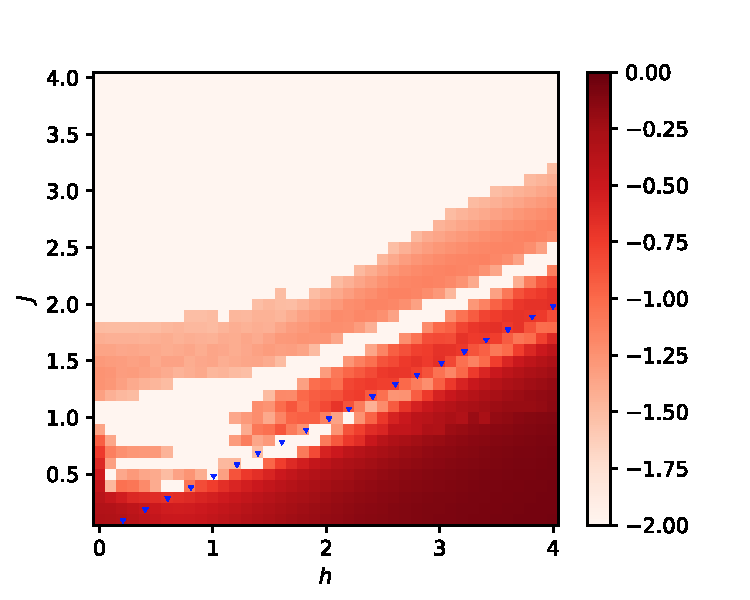
\includegraphics[width=0.7\textwidth]{./scar/scar1.pdf}
\bicaption{初态为$|Z_2\rangle$的局域算符时间平均期望值与吉布斯系综平均期望值之差。选取不同的链长$L=10,12,14,16,18$,我们做有限尺寸修正。然后对两种平均的期望值做差取绝对值后再画在10为底的对数坐标下。我们选取截断$\Delta=0.03$作为临界值,绝对值低于临界值的我们在图中用白色表示。蓝色三角标记$J=\frac{h}{2}$。}{Difference between long time average and Gibbs canonical ensemble average of local operator $\hat{L}=\hat{\sigma}_1^z\hat{\sigma}_2^z$ under $|Z_2\rangle$ initial state. By choosing different length of chain $L=10,12,14,16,18$, we do finite size scaling to obtain $L=\infty$ result. We choose critical difference between two average to be $\Delta=0.03$. When $|\Delta|<0.03$, we mark as white color to represent thermalization. Blue triangles mark special line $J=\frac{h}{2}$. }
\label{scarphasediag}
\end{figure}
%***********************************

我们将相图分为几个区域来讨论:


\subsection{Many body scar区域}
首先是多体伤痕区域,对于里德堡哈密顿量,带入$\hat{n}_i = \frac{\hat{\sigma}_i^z+1}{2}$:
\begin{equation}
\begin{split}
	\hat{H}_{Rydberg}(V) &= \sum_{i=1}^{L} \hat{\sigma}_{i}^{x} + V \sum_{i}^{L} \hat{n}_i\cdot\hat{n}_{i+1} \\
	\quad &= \sum_{i=1}^{L} \hat{\sigma}_{i}^{x} + \frac{V}{4}  \sum_{i}^L \hat{\sigma}_i^z\hat{\sigma}_{i+1}^z + \frac{V}{2} \sum_i^L \hat{\sigma}_i^z  + \frac{V}{4} \sum_i^L \hat{1} \\
\end{split}
\end{equation}
我们发现如果在$\hat{H}_{Ising}(g,J,h)$中取$g=1,J=V/4,h=V/2$,则两者是等价的(仅相差一个与链长有关的常数):
\begin{equation}
\hat{H}_{Ising}(g=1,J=\frac{V}{4},h=\frac{V}{2}) = \hat{H}_{Rydberg}(V) + C
\end{equation}
因此在带有纵场的横场伊辛模型中,如果沿着$J=h/2$这条特殊的线来看,在$J$较大的极限下,有效模型为PXP模型,。

如果我们把$J=h/2$这条线从相图里摘出,我们就得到了里德堡哈密顿量,对应$V=4J$,如图~\ref{scar1_2}~(a)所示。沿着$J=h/2$这条线,当$J\ll 1$处于弱耦合的时候,此时由于靠近单自旋极限,从$|Z_2\rangle$出发的动力学具有非热化的行为是可以期待的。当$J\gg 1$处于强耦合的时候,此时为PXP极限,基态子空间对应没有近邻格点同时处于$\uparrow$,有效模型为:
\begin{equation}
	\hat{H}_{PXP} = \sum_i\hat{P}_{i-1}\hat{\sigma}_{i}^x\hat{P}_{i+1}
\end{equation}
其中$\hat{P}_i=|\downarrow\rangle\langle\downarrow|$,从$|Z_2\rangle$作为初态出发,会观察到局域算符期望值的持续震荡行为,其长时间系综平均不等于热力学系综平均,此即量子多体伤痕动力学。这是违背本征热化假说的反常动力学。在中间区域$h\sim 1$,我们看到由于时间平均随着$J$的变化存在一极大值结构,导致仅在与热力学吉布斯正则系综平均曲线的两个交点处有局域算符的时间平均与系综平均之差为0,在其余情况下局域算符期望的时间平均不等于系综平均。随着$J$从0开始增大,体系逐渐远离单自旋极限,同时局域算符的时间平均与热力学系综平均的差值在缩小,但是随着$V=4J$慢慢增大,PXP有效模型开始涌现,再一次使得局域算符的时间平均期望值远离了其热力学系综平均期望值。对于这一连续的渡的过程,我们展示更多的细节我们分别取三个不同的参数区间下计算与本征态与初态的投影、半链纠缠熵与实际动力学,如图~\ref{scar1_2_detail}~所示:
%***********************************
\begin{figure}[h]
\centering
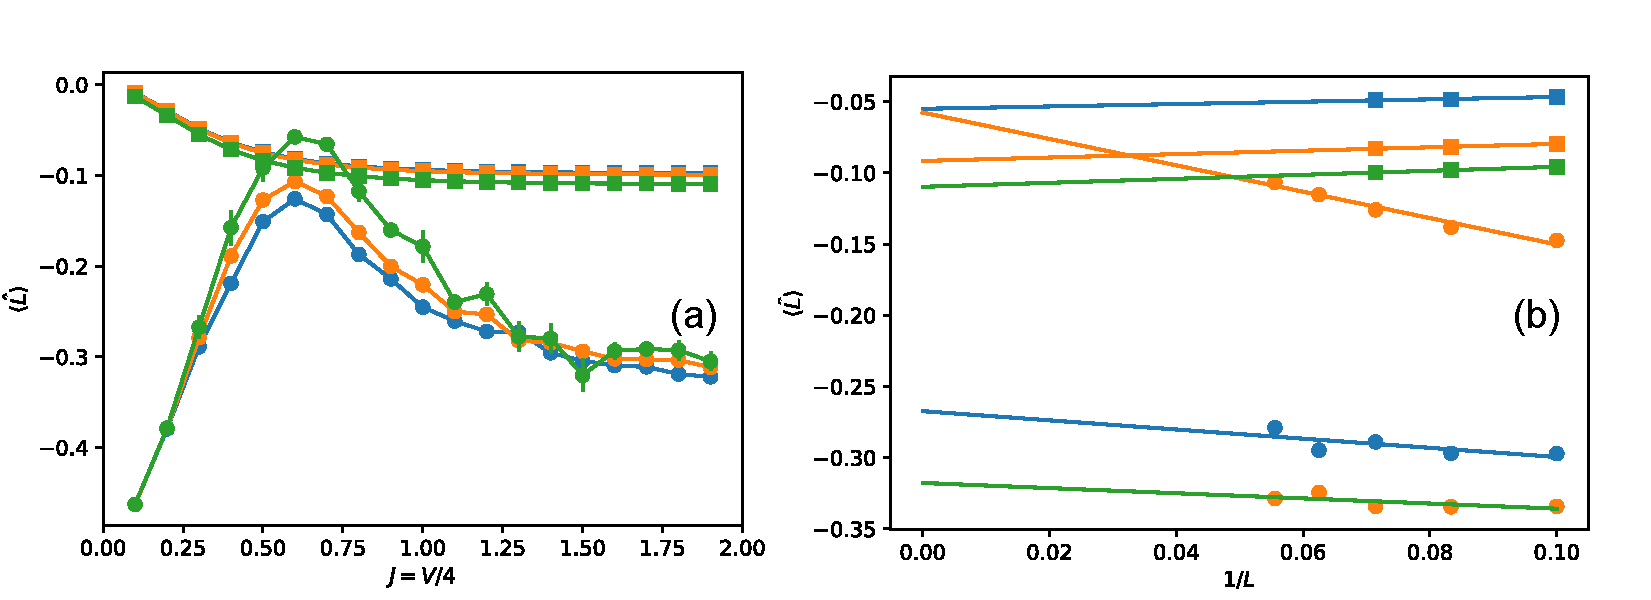
\includegraphics[width=0.9\textwidth]{./scar/scar2.pdf}
\bicaption{图(a)为沿$J=h/2$特殊比例下局域算符$\hat{L}=\hat{\sigma}_1^z\hat{\sigma}_2^z$时间平均(圆点)与系综平均(方点),其中蓝色点为$L=14$,橘色点为$L=18$,绿色点为有限尺寸修正结果,带有线性拟合的误差。图(b)为$J=0.3$(蓝色),$J=0.6$(橘色),$J=2.5$(绿色)下的有限尺寸修正,圆点代表时间平均,方点代表吉布斯系综平均。}{ Fig (a) for time average(dots) and Gibbs canonical ensemble average(square points) of local operator $\hat{L}=\hat{\sigma}_1^z\hat{\sigma}_2^z$ under $|Z_2\rangle$ initial state, blue points for $L=14$, orange points for $L=18$ and green points for result of finite size scaling with error bar of linear fitting. Fig (b) for finite size scaling of time average(dots), Gibbs canonical ensemble average(square points) and linear scaling fitting (solid lines) under $J=0.3$(blue), $J=0.6$(orange), $J=2.5$(green). }
\label{scar1_2}
\end{figure}
%***********************************
从图(a,b)中我们可以看到,在弱耦合以及中间区域,与初态$|Z_2\rangle$交叠较大的本征态中,都会有一些反常低熵态。此时能谱尚未发生片段化(以相邻的$\uparrow\uparrow$的数目来分隔不同的片段),这些反常低熵态处于能谱中靠近基态的位置,正是由于这些反常低熵态的存在导致这一非热化行为的出现,其动力学如图(d,e)所示。在图(c,f)中我们进一步展示了PXP极限下的情况,在这一极限下这些由于能谱完全发生片段化,仅考虑最低子空间中(没有$\uparrow\uparrow$),与初态$|Z_2\rangle$交叠较大的本征态中仍然会出现反常低熵态,这些反常低熵态有规律的近似等间距分布,导致局域算符动力学中具有清晰的非热化震荡行为。
%***********************************
\begin{figure}[h]
\centering
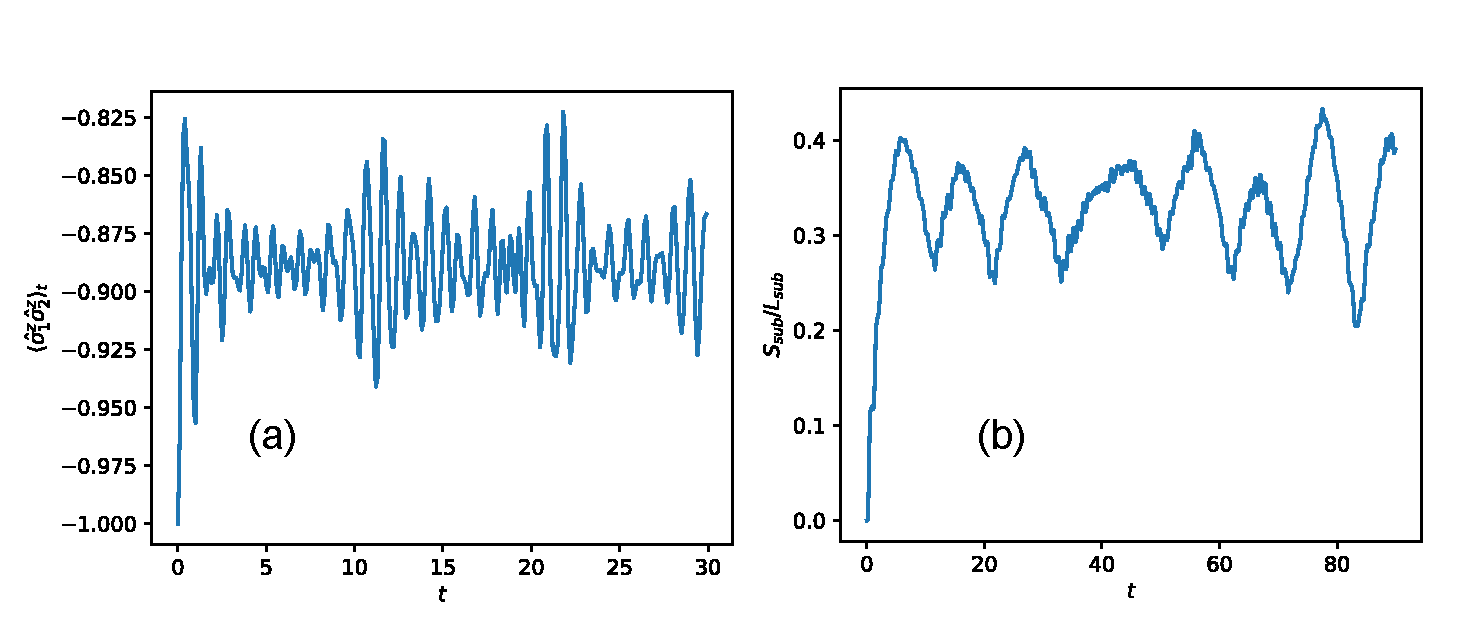
\includegraphics[width=1.2\textwidth]{./scar/scar3.pdf}
\bicaption{图(a,b,c)中散点代表与初态$|Z_2\rangle$的投影权重,颜色代表半链纠缠熵,蓝色虚线代表初态能量平均值。不同参数$J$下的本征态到初态投影权重、半链纠缠熵、演化动力学。其中(a)对应$J=0.3,h=0.6$,(b)对应$J=0.6,h=1.2$,(c)对应$J=2.5,h=5$。图(d,e,f)代表不同$J$下从初态为$|Z_2\rangle$出发的局域算符动力学。橘黄色虚线代表有限尺寸修正后$\hat{L}$的热力学吉布斯正则系综平均。我们取$L=16$}{Fig (a, b, c) for overlap between initail state and eigenstate, entanglement entropy of half chain and local operator dynamics under $|Z_2\rangle$ initial state. Fig (a) for $J=0.3,h=0.6$, Fig (b) for $J=0.6,h=1.2$ and Fig (c) for $J=2.5,h=5$. Scatterd dots for overlap and color bar for entanglement entropy of half chain. Blue dashed lines in Fig (a, b, c) for expectation energy of $|Z_2\rangle$. Fig (d, e, f) for dynamics of $\hat{L}=\hat{\sigma}_1^z\hat{\sigma}_2^z$ under different J starting from $|Z_2\rangle$.  Orange dashed lines in Fig (d, e, f) for Gibbs canonical ensemble average of $\hat{L}$ after finite size scaling. We choose $L=16$.}
\label{scar1_2_detail}
\end{figure}
%***********************************

%***********************************
\begin{figure}[h]
\centering
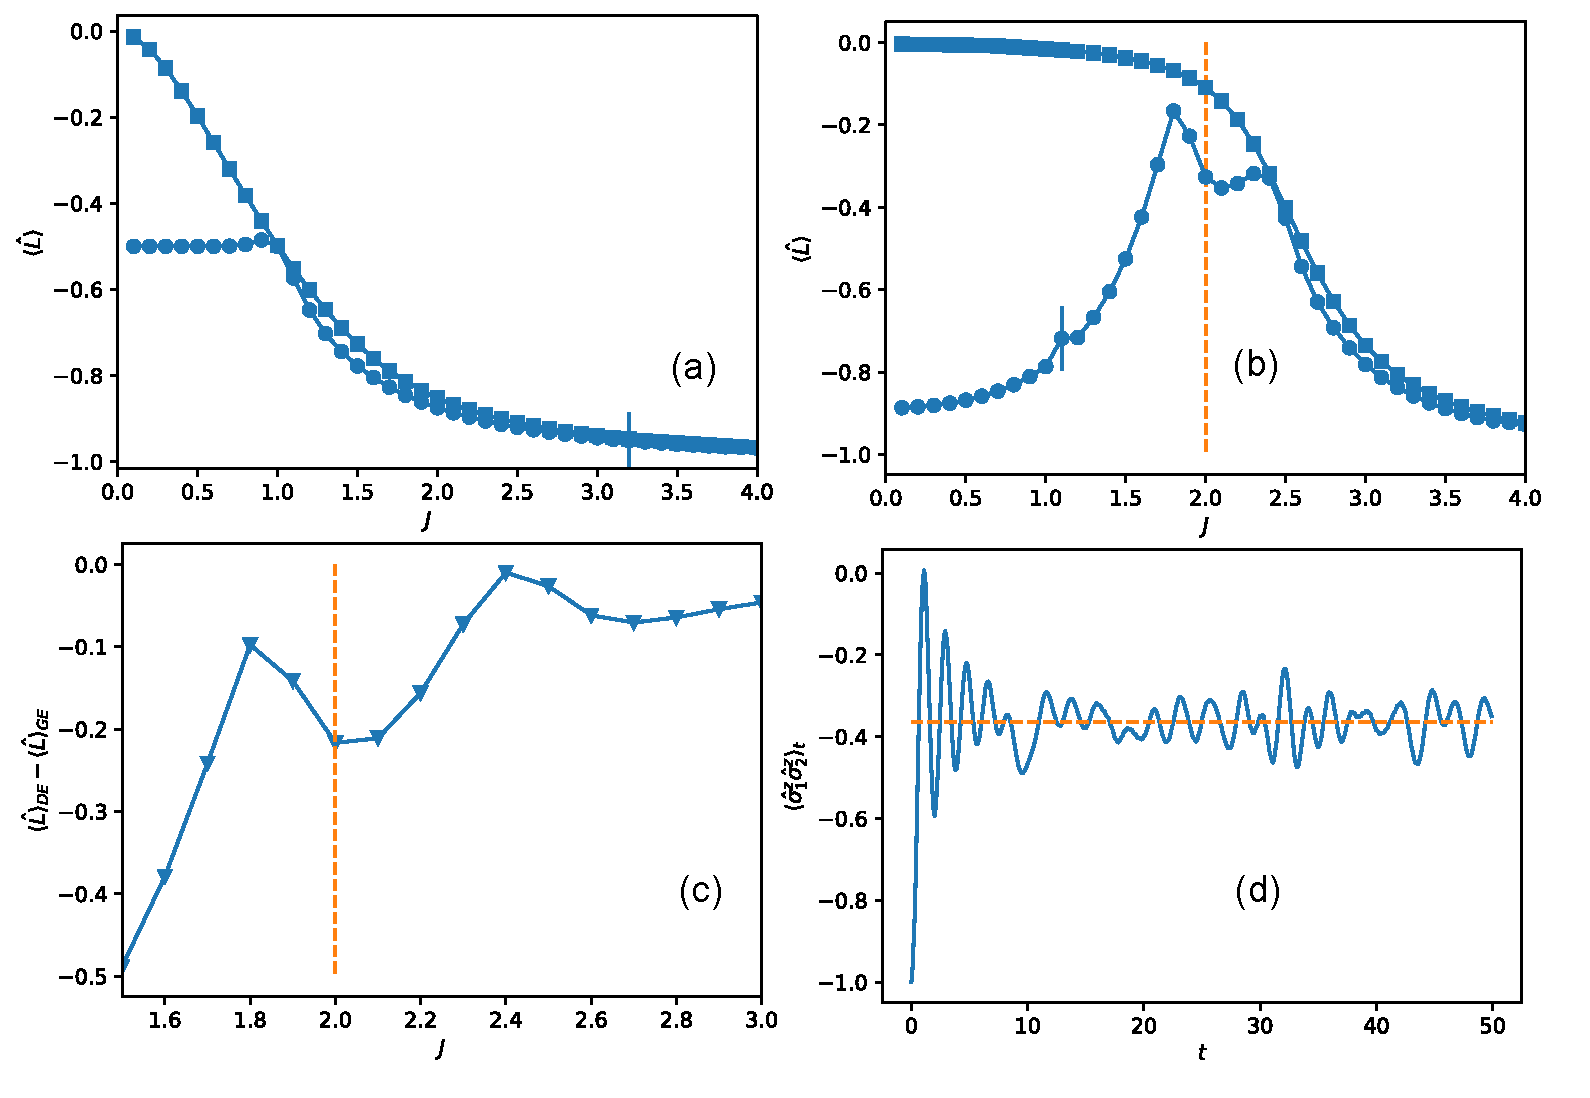
\includegraphics[width=0.8\textwidth]{./scar/scar4.pdf}
\bicaption{图(a,b)为局域算符$\hat{L}=\hat{\sigma}_1^z\hat{\sigma}_2^z$自初态$|Z_2\rangle$出发动力学的时间平均与热力学吉布斯正则系综平均之差。图(a)为$h=0$,图(b)为$h=4$。图(b)中橘黄色虚线代表$J=h/2$处。图(c)为实际的动力学演化。其中橘黄色虚线代表有限尺寸修正后的热力学吉布斯正则系综平均。我们取$L=16$。}{Fig (a, b) for difference between time average and Gibbs canonical ensemble average of local operator $\hat{L}=\hat{\sigma}_1^z\hat{\sigma}_2^z$ under $|Z_2\rangle$ initial state. Fig (a) for  $h=0$ and Fig (b) $h=4$. Orange dashed line in Fig (b) for $J=h/2$. Fig (c) for dynamics of local operator $\hat{L}=\hat{\sigma}_1^z\hat{\sigma}_2^z$ starting from $|Z_2\rangle$ under $J=2.4,h=4$. Orange dashed line in Fig (c) for Gibbs canonical ensemble average of local operator after finite size scaling. We choose $L=16$. }
\label{h04}
\end{figure}
%***********************************
在上述沿着$J=h/2$的特殊比例下,我们分析了相图的热化性质。进一步我们在PXP极限下,改变这一$h:J$的比例,探索不同$J$带来的影响,此时我们选取足够大的$h=2$,对于$J=h/2+a$,则在$h,J\gg a$的区域:
\begin{equation}
\begin{split}
\hat{H}_{Ising}&=\sum_i\hat{\sigma}^x_i + J\sum_{i}\hat{\sigma}^z_i\sigma^z_{i+1} + 2(J-a)\sum_{i}\hat{\sigma}^z_i  \\
\quad &= \sum_i\hat{\sigma}^x_i + 4J\sum_{i}^{L} \hat{n}_i\cdot\hat{n}_{i+1} - 2a\sum_{i}\hat{\sigma}^z_i  + C\\
\end{split}
\end{equation}
额外纵场项会变成PXP模型中的$h_{eff}\sum_i\sigma^z_i = -2a\sum_i\sigma^z_i$,物理意义相当于在PXP模型中再加一个沿$z$方向纵场,即:
\begin{equation}
\hat{H}_{eff} = \sum_{i}^{L} \hat{P}_{i-1}\hat{\sigma}_i^x\hat{P}_{i+1} + h_{eff}\sum_i\hat{\sigma}^z_i 
\end{equation}
在图~\ref{h04}~(b)中我们给出这一PXP极限附近加有效磁场的时间平均与热力学吉布斯正则系综平均,在图~\ref{h04}~(c)中我们给出两种平均的差值。随着a的增大,$h_{eff}<0$,首先会破坏多体伤痕动力学,使其先热化,大约在$a_c=0.4$附近,此时多体伤痕动力学被完全破坏,此时动力学如图~\ref{h04}~(d)所示,这一现象在最近的研究中已经被发现\cite{Yao2022quantum}。如果反向增加磁场及$h_{eff}>0$,我们也会看到这一非单调的行为,表明多体伤痕动力学反常行为被抑制,但是并没有被彻底破坏,如图~\ref{h04}~(c)所示。

而在$h=0$时,此时为严格可解的横场伊辛模型,此时我们展示这一严格可解系统的时间平均与热力学系综平均,如图~\ref{h04}~(a)所示。可以看到仅在$J=1$时间平均等于系综平均,对于这样的严格可解模型,通常用广义吉布斯系综给出整个$J$区间的广义热化预测\cite{vidmar2016generalized}。而在$J\gg 1$极限下,系统进入特殊的弱热化区间。



\subsection{弱热化区域}
在相图的上半部分,此时$J \gg \frac{h}{2}$,当$g=0$时,我们有$|Z_2\rangle=|10101010...\rangle$与$|Z'_{2}\rangle=|0101001...\rangle$为系统的两个简并基态。但是着两个简并基态无法通过动力学联系起来。当$g\neq 0$时候,打开量子涨落,动力学局限在基态以及基态附近的准粒子激发附近。此时的准粒子激发主要有两类,近似为$|...00...\rangle$
与$|...11...\rangle$,对应的准粒子能量为$4J-2h$与$4J+2h$,当初态处于$|Z_2\rangle$时,此时的动力学即由准粒子决定的弱热化动力学。其震荡频率反映的是准粒子的能量,其振幅由$\sum_i \hat{\sigma}_i^x$引发的量子跃迁决定,如图~\ref{weak}~所示,同时单自旋的熵远低于$ln2$并伴有明显的震荡行为。
%***********************************
\begin{figure}[h]
\centering
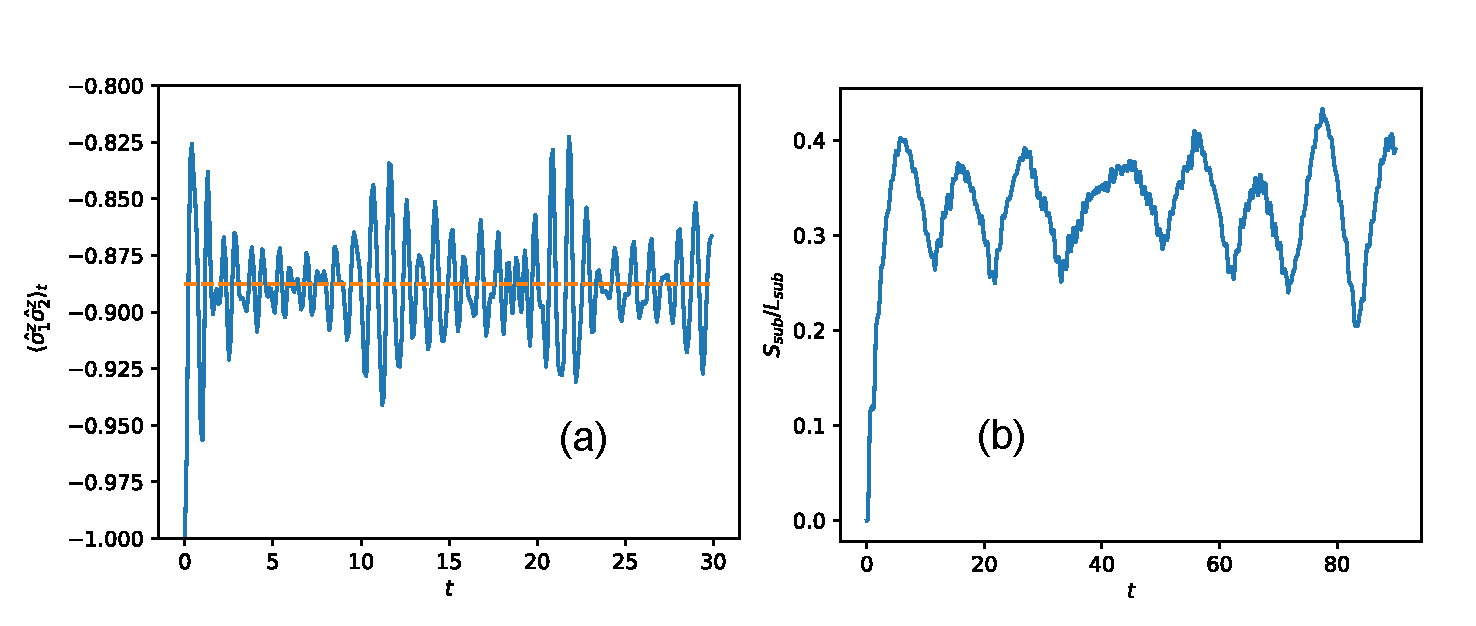
\includegraphics[width=1.0\textwidth]{./scar/scar5.pdf}
\bicaption{图(a)代表初态为$|Z_2\rangle$的动力学演化,橘黄色虚线代表有限尺寸修正后下的热力学吉布斯正则系综平均。图(b)为第一个格点的纠缠熵随时间的变化。我们选取$L=16, J=2.3, h=1.1$。}{Fig (a) for dynamics of local operator $\hat{L}=\hat{\sigma}_1^z\hat{\sigma}_2^z$ starting from$|Z_2\rangle$. Orange dashed line for Gibbs canonical ensemble average of after finite size scaling. Fig (b) for entanglement entropy dynamics of spin degree on first site. We choose $L=16, J=2.3, h=1.1$ for simulation.}
\label{weak}
\end{figure}
%***********************************

最后在中间区域$h\sim 1, J \sim 1$附近,我们从$|Z_2\rangle$出发的动力学结果表明此时热化仍然是很慢的,其行为类似于之前观测到的弱热化行为,与此时选取初态为$|Y-\rangle = |Y-\rangle_0 \otimes|Y-\rangle_1\otimes |Y-\rangle_2 \otimes... $的热化动力学有很大不同,局域算符与单自旋纠缠熵的动力学中表现出明显强于强热化行为的震荡,单自旋熵的上界为$ln2$,如图~\ref{midweak}~所示。

\section{小结}\label{4sec:sum}
我们选取$|Z_2\rangle$作为初态,进行长时间动力学平均与热力学系综平均的比较,发现这一初态对应的热化相图。首先多体伤痕物理附近,对应$J:h=1:2$,在整个耦合区间我们发现时间平均都不等于系综平均。在这一特殊比例附近,对应在PXP模型下加入沿z方向的磁场,这一磁场沿正向和反向都会抑制反差的多体伤痕动力学,但仅在$h_{eff}<0$的时候会彻底破坏。在$J\gg h/2$的弱热化区域下,我们观察到了靠近基态带来的弱热化动力学,并给出简单的准粒子激发解释。最后在中间区域,我们也观测到了弱热化的迹象,并与此时强热化的动力学做了对比,其中单自旋熵的震荡行为揭示了这一点。



%***********************************
\begin{figure}[h]
\centering
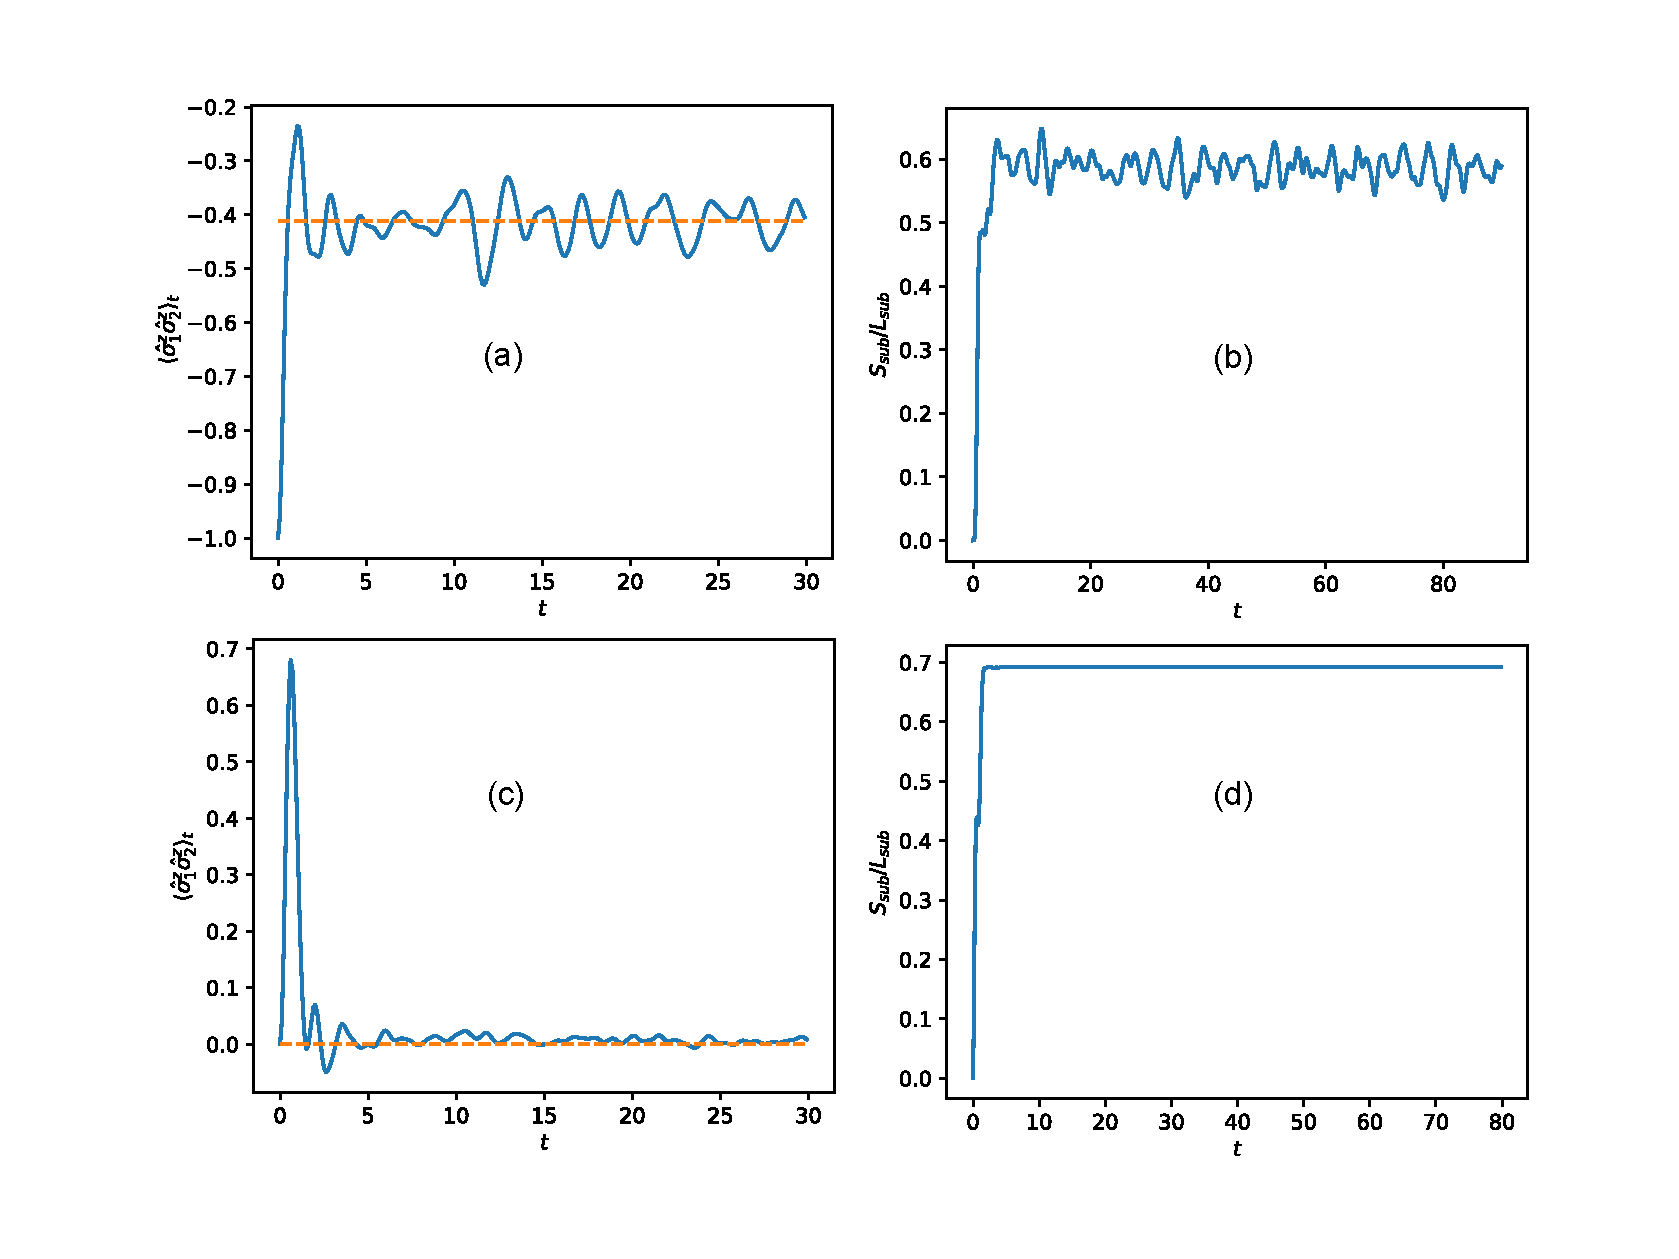
\includegraphics[width=1.0\textwidth]{./scar/scar6.pdf}
\bicaption{图(a,b)为$J=0.9,h=0.8,L=16$下初态为$|Z_2\rangle$的局域算符$\hat{L}=\hat{\sigma}_1^z\hat{\sigma}_2^z$动力学演化(a)与第一格点纠缠熵的动力学演化(b)。图(c,d)为同参数下初态为$|Y-\rangle$的局域算符$\hat{L}=\hat{\sigma}_1^z\hat{\sigma}_2^z$动力学演化(c)与第一格点纠缠熵的动力学演化(d)。橘黄色虚线代表有限尺寸修正后的热力学吉布斯正则系综平均。}{ Fig (a, b) for dynamics of local operator $\hat{L}=\hat{\sigma}_1^z\hat{\sigma}_2^z$(a) and entanglement entropy of spin degree on first site(b) starting from $|Z_2\rangle$. Fig (c,d ) for dynamics of local operator $\hat{L}=\hat{\sigma}_1^z\hat{\sigma}_2^z$(c) and entanglement entropy of spin degree on first site(d) starting from $|Y-\rangle$. We choose $L=16, J=0.9, h=0.8$ for simulation. Orange dashed lines in Fig (a, c) for Gibbs canonical ensemble average after finite size scaling.}
\label{midweak}
\end{figure}
%***********************************







